\chapter{Work on the Thesis} \label{chap_process}

This chapter explains the procedure for writing a thesis at THL. 

\section{Thesis registration form}

Approx. three weeks in advance of the start it is necessary to begin the process to check the fulfillment of requirements for writing a thesis at the secretariat. The student can either fill out a form at the secretariat directly or can ask via e-mail to ei@th-luebeck.de to perform the checks. This does not mean that the student is immediately registered for the thesis, it is just a check of requirements. If all requirements are fulfilled with respect to the examination regulations, the first advisor will get a notification (with CC to the student). The first advisor then provides the title, official start date, and may also provide a task description. This official start date determines the final thesis hand-in date three months later (six months in case of master thesis).

First advisor of a thesis can in general be any member of the faculty as long as the scientific area of this person matches to the topic of the thesis. For some members of the faculty who are not professors it is necessary that their role as first advisor is confirmed by the examination board.

Remark for Chinese students: Since all Chinese students start their theses on the same day, a special procedure applies. Please note the remarks on this in the lecture of Ms. Hanesova.

\section{Specification of a thesis subject}

Several situations are possible for finding a thesis topic.

\subsection{Given topic}

It is possible that the first advisor already has a clear idea about a subject. She or he may already provide a title and also a description of the task. Nevertheless, a discussion of the subject and the tasks should take place between student and first advisor. It is possible to change or improve the task description as a consequence of this discussion. The student should verify together with the first advisor that those aspects as discussed in Section \ref{sec_newtopic} have been taken into account. 

Remark: This is the typical situation for Chinese students doing their work inside of THL.

\subsection{Joint specification of a topic} \label{sec_newtopic}

For theses where the student has a proposal for a subject (which is often the case for theses in cooperation with companies) it is necessary to jointly specify a task description. The proposal for the topic and task description draft should be provided in a written manner by the student. One or two pages are sufficient for that. The (potential) first advisor should get the possibility to judge from the description whether the topic is suited for a thesis. The description should comprise a draft for an outline. 

The following aspects are relevant for the task description:
\begin{itemize}
\item The choice of the subject needs to reflect a suitable challenge and effort. On the one hand, this means that the topic for a bachelor thesis has to be appropriate to address it within three months. These three months have to be sufficient even if unexpected difficulties arise (e.g. hard to find programming errors; unclear requirements which become apparent later). On the other hand, the topic needs to require knowledge which has been gained throughout the studies. Very often a combination of theoretical considerations combined with a (prototypical) practical implementation is chosen. A task description which means just an implementation of given concepts would be regarded as not sufficiently demanding.  
\item The task description together with the outline needs to address the following questions: 
  \begin{itemize}
  \item What is the main problem? It should be tried to answer this question precisely in one or two sentences.
  \item Why is it important to find a solution for the problem?
  \item Why are existing solutions regarded as insufficient?
  \item How is the way to address the problem? 
  \item How can it be checked (later on) whether the developed solution actually solves the problem? This is typically done by a catalog of criteria which needs to be developed first.
  \end{itemize}
\item The thesis has to match with scientific standards also in cases where the thesis is done in collaboration with an external company. The steps which are taken in the course of the thesis need to have technical reasons. An argumentation that a certain way to address a problem is desired by senior employees is not allowed. The thesis needs to be approached in an objective manner and not with respect to the company's views. This is also necessary for the written thesis where it is unacceptable to repeat advertisement messages of the company (e.g. ``company X the worldwide leader in manufacturing of product Y ...''). 
\item The student should consider her or his own professional future in the cooperation with the company. For instance, it should be taken into account whether work similar to the one conducted throughout the thesis is also interesting for the student on the long run. The choice of the topic will be subject of hiring talks in the future and can be helpful to show skills in an area that matches to the offered job.
\item The task description and title of the thesis need to be considered carefully so that it is possible to get a clear idea of the topic, but also to show that it is a challenging topic. It is important to note that the title is chosen at the beginning and cannot be changed afterwards.
\end{itemize}

The official task description is derived from the proposal as Word or simple text file in collaboration with the first advisor.

For many theses there is a preparation of the work in front of the official registration of the thesis. This is a common procedure in particular in the collaboration with companies.

Remark for Chinese students: Due to the strict time line a preparation of work is only possible in February and March in front of the official registration in the second half of March.

\section{Registration form back to secretariat (via first advisor)}

Based on the task description which is provided on the form the secretariat derives the official task description. The official source of the topic and task description is the examination board represented by its head. The student does not write anything on the form. A request to fetch the official task description is sometimes provided by paper mail.

\section{Thesis duration}

The thesis has to be finished until a predefined date and needs to be completed with respect to the required formalities. The duration of a bachelor thesis is three months. A master thesis takes six months.

\section{Advice}

There are differences between the advice for internal and external theses.

\subsection{Advice for an internal thesis}

For the advice on internal theses it is common to agree on weekly or biweekly meetings. It is sufficient in many cases if conducted and future work is discussed orally.

\subsection{Advice for an external thesis}

For an external thesis in a company short written reports which are sent via e-mail are better suited. They may be sent for a time interval of three weeks for example. For those reports the following outline is suitable: Student name, thesis title, report date, report interval, status (e.g.~implementation, measurements, calculations, or simulation), results (same category, but concrete work, e.g. finished prototype platform), documentation (specific information, e.g.~finished related work chapter), plan for the next time interval (specific information like: measurement preparation in the next week, conducting of measurements in the following week, finish measurement report in the third week). Those short reports are helpful for planning and for the early detection of timing issues.

During the work at an external company the first advisor will visit the students as needed. The agreement on the date of the visit is usually done via e-mail. 

\subsection{Intermediate versions of the thesis}

The student sends intermediate versions of the thesis to the advisor. This holds both for internal and external theses. The student should use version numbers in an obvious way and should mark for the advisor which parts of thesis are new or have been revised significantly. This is eases the correction work for the advisor. 

\section{Second advisor}

Approx.~four weeks before the end of the work on the thesis the student should get in contact with a second advisor. The second advisor should be familiar with the scientific area to which the subject of the thesis is related. The first advisor can be asked for help to recommend a second advisor.

Important: The student has to take care of the coordination of dates.

\section{Deadline and submission}

The submission of the demanded \textbf{two hard copies} can be done by personal delivery to the secretariat or be done via paper mail (address: Technische Hochschule L�beck, Fachbereich Elektrotechnik und Informatik, Pr�fungsausschuss, M�nkhofer Weg 239, 23562 L�beck, Germany). In the second case, the postmark stamp fixes the submission date. In addition to the written thesis the thesis itself and further material (program code, etc) has to be put on a CD and has to be attached to each hard copy (inside of the back cover). One of the hard copies will be archived later. The second one is checked by the first advisor and will remain in her or his office. 

The \textbf{deadline} has to be met in any case since the thesis is regarded as \textbf{failed} otherwise. An exception is only possible in case of third party mistakes (e.g.~if the external company has not delivered important documents as promised) or in case of illness. In these situations a request for a prolongation of the thesis duration has to be posed in front of the expiry of the submission date. A deadline extension due to an inaccurate time organization of the student is not possible. The topic of the thesis may be returned once within the first one-third of the thesis duration. This has to be stated in a written manner towards the examination board. If the thesis is regarded as ``failed'' at the end, a second attempt (but no third attempt) is possible (the request for doing a second attempt has to be posed within the next two semesters). 

The submitted thesis copies must be printed and bound to archives. The binding can be done in the print office in building 36, but also in town. Students should not have the thesis bound until the supervisor has approved the final draft, including all extra pages both preceding and following the main text. There are two types of binding available as illustrated in Figure \ref{fig:bindings}. Both simple binding and hard binding are allowed. However, it is a good idea to ask the supervisor for her or his choice. The student should make sure that all pages are there and that they have the right order.

%Figure from PNG-File - take care that the figure has a sufficient resolution (so that a scaling >300dpi can be used in the printout) 
\begin{figure}[htb]
  \centering
  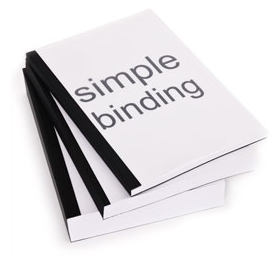
\includegraphics[width=.4\textwidth]{simple_binding} % PNG-File
	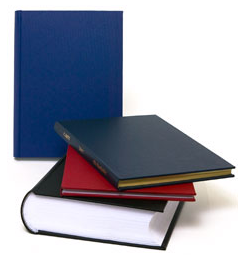
\includegraphics[width=.4\textwidth]{hardcover}\\ % PNG-File
  \caption{Simple binding (left) and hard cover (right) \cite{coll13}}\label{fig:bindings}
\end{figure}

Sometimes it is useful to make more hard copies, e.g.~for employees from companies where the thesis work has been done.

Remark for Chinese students: Please consider that the same deadline holds for the other students as well. Therefore, queues are possible if everyone wants to print the thesis on the same day.

\section{Finding an oral examination date}

The student should agree with the advisors on the date, time and place of the oral examination (called ``colloquium'') well in advance. Dates outside of the lecture weeks can be hard to arrange. The student should ask the advisor about her or his ideas on the course of the colloquium (exact duration of the presentation, use of media, short demonstration possible).

\section{Colloquium}

The student prepares a slide set for the colloquium which is designed to take 25 minutes to be presented (deviations are possible in particular for online degree programs, check with first advisor). It is estimated that it takes two or three minutes to present a single slide so that approx.~10 slides should be used. Spelling mistakes on the slides should be avoided. The presentation may include the use of a blackboard, the showing of physical prototypes or a short demonstration.

The focus of the slides should be the work that the student has done. This means that it is inappropriate to spend too much time on explaining the background or discuss related work. Often the student can use a similar outline as the one used in the written thesis. An important difference is that the presentation should not strive for completeness, but can select specific examples. A file with advice on the colloquium slides can be found in the folder about the presentation.

The colloquium itself takes place in a seminar room or a small lecture room. During the time of the presentation the public can participate, but the public is excluded when the advisors pose their questions. It is a pity that the colloquium often takes place without additional listeners which is inappropriate in relation to the effort that is invested into many theses. The student should check the availability of the technical equipment in advance. She or he should be in the room on time to cope with (frequent) difficulties, e.g. that the beamer does not want to cooperate with the notebook, and to resolve them before the start of the colloquium.

At the end of the colloquium the presentation should be delivered to the first advisor.
 
\endinput 